\chapter{Previous work}

This project sits at the intersection of two areas of research. 
First there is the application of \Gls{ai} in medical applications, specifically for segmentation problems.
Then, there is the active area of research of \Gls{weaklysupervisedl} machine learning.

\section{Medical segmentation problems}

\Gls{ai} has proven to be a valuable contribution to medical practice to reduce the burden of repetitive tasks on the medical caregiver.

\todo[inline]{elaborate: ppg to blood pressure - slaapapnue}

For segmentation tasks, the U-net \cite{Ronneberger2015} is widely used. 
This architecture can be represented by a characteristic U-shape, as the name indicates.
It consists of 

\begin{SCfigure}[][htb]
    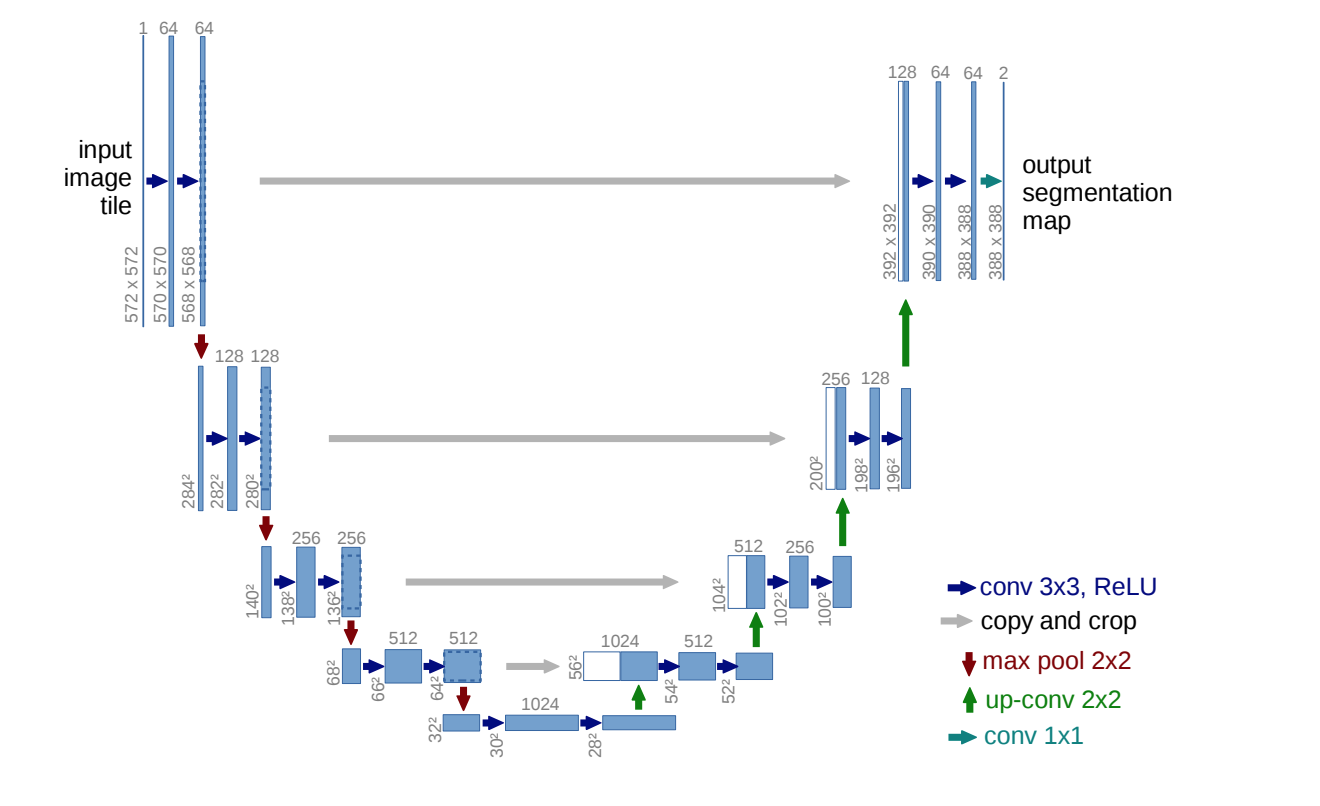
\includegraphics[width=10cm]{/home/thesis/images/UNet_Ronneberger.png}
    \caption{U-Net architecture, as illustrated in \cite{Ronneberger2015}. 
    Each blue box represents a multi-channel feature-map. 
    The number of channels is indicated above the box, the $x \times y$ dimensions are indicated at the bottom left.
    The gray arrows indicate the feature maps in the contracting path are copied and concatenated to the feature maps of the expanding path.}
    \label{fig:unet}
\end{SCfigure}



\section{Weakly supervised segmentation}

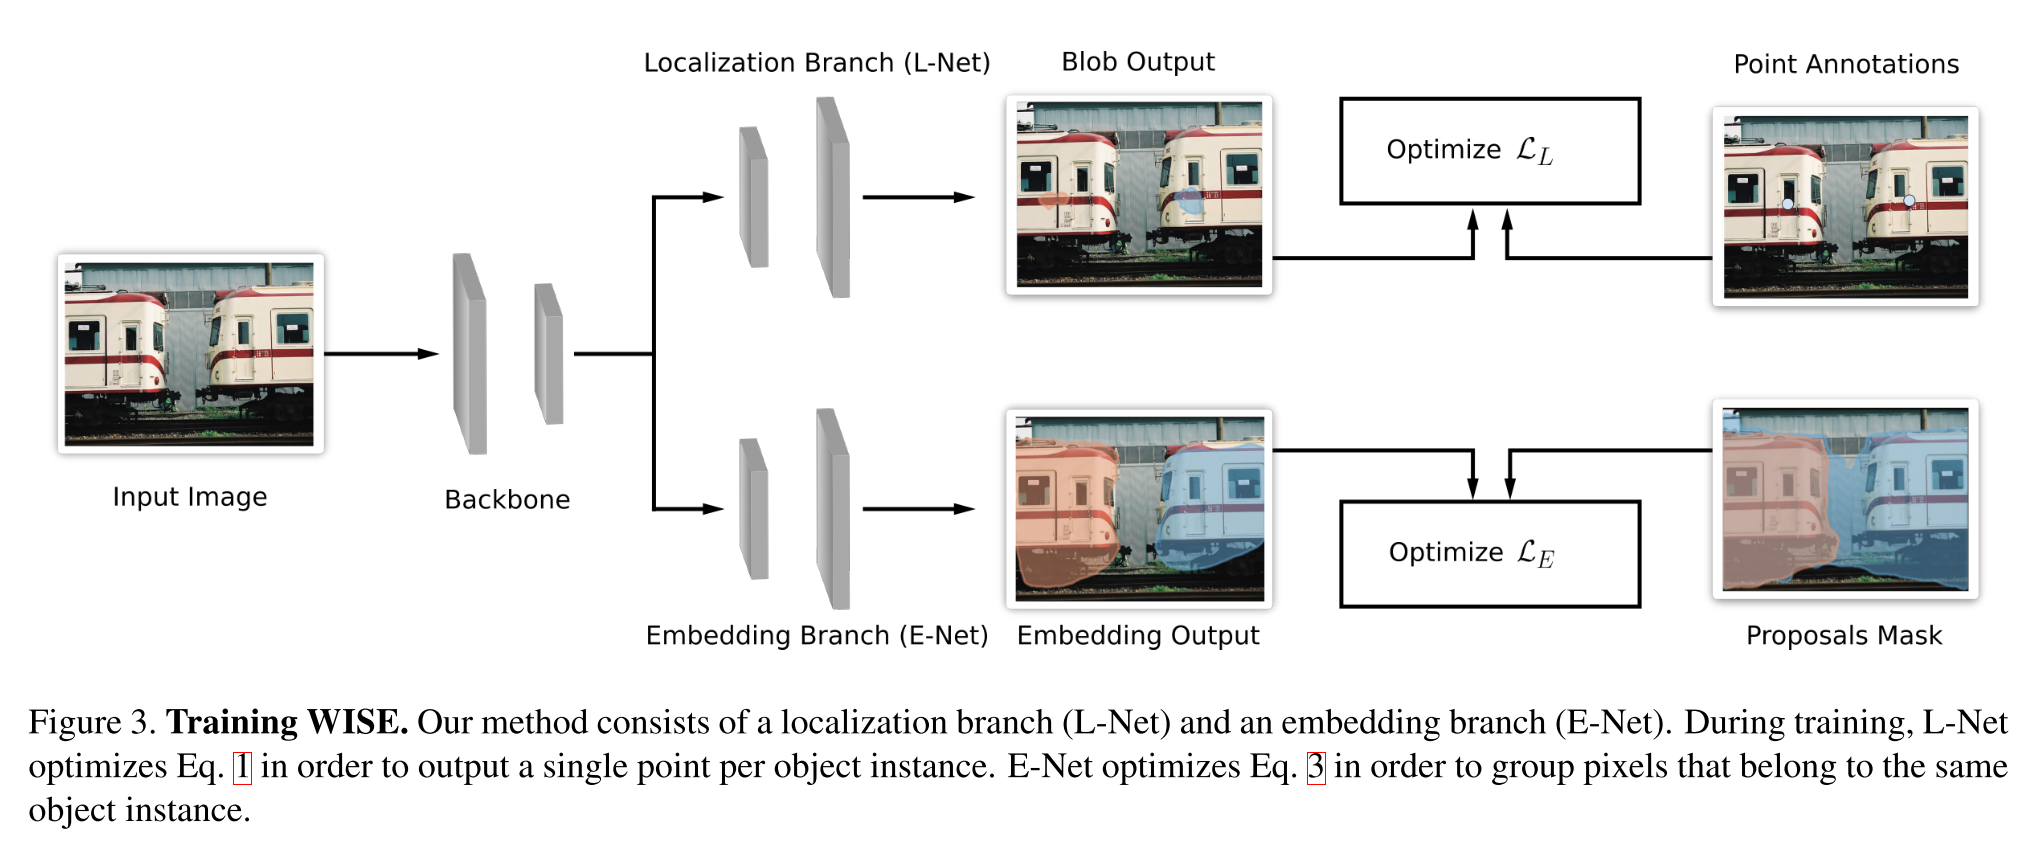
\includegraphics[width=10cm]{/home/thesis/images/Laradji_architecture.png}
\captionof{figure}{Architecture of the U-net based segmentation}
\label{fig:laradji}